\documentclass{article}

\usepackage{fancyhdr}
\usepackage{extramarks}
\usepackage{amsmath}
\usepackage{amsthm}
\usepackage{amsfonts}
\usepackage{tikz}
\usepackage[plain]{algorithm}
\usepackage{algpseudocode}
\usepackage{mdframed}
\usepackage{listings}
\usepackage{color}
 
\definecolor{codegreen}{rgb}{0,0.6,0}
\definecolor{codegray}{rgb}{0.5,0.5,0.5}
\definecolor{codepurple}{rgb}{0.58,0,0.82}
\definecolor{backcolour}{rgb}{1,1,1}

\usetikzlibrary{automata,positioning}

%
% Basic Document Settings
%

\topmargin=-0.45in
\evensidemargin=0in
\oddsidemargin=0in
\textwidth=6.5in
\textheight=9.0in
\headsep=0.25in

\linespread{1.1}

\pagestyle{fancy}
\lhead{\hmwkAuthorName}
\chead{\hmwkClass\ (\hmwkClassInstructor\ \hmwkClassTime): \hmwkTitle}
\rhead{\firstxmark}
\lfoot{\lastxmark}
\cfoot{\thepage}

\renewcommand\headrulewidth{0.4pt}
\renewcommand\footrulewidth{0.4pt}

\setlength\parindent{0pt}

%
% Create Problem Sections
%

\newcommand{\enterProblemHeader}[1]{
    \nobreak\extramarks{}{Problem \arabic{#1} continued on next page\ldots}\nobreak{}
    \nobreak\extramarks{Problem \arabic{#1} (continued)}{Problem \arabic{#1} continued on next page\ldots}\nobreak{}
}

\newcommand{\exitProblemHeader}[1]{
    \nobreak\extramarks{Problem \arabic{#1} (continued)}{Problem \arabic{#1} continued on next page\ldots}\nobreak{}
    \stepcounter{#1}
    \nobreak\extramarks{Problem \arabic{#1}}{}\nobreak{}
}

\setcounter{secnumdepth}{0}
\newcounter{partCounter}
\newcounter{homeworkProblemCounter}
\setcounter{homeworkProblemCounter}{1}
\nobreak\extramarks{Problem \arabic{homeworkProblemCounter}}{}\nobreak{}

%
% Homework Problem Environment
%
% This environment takes an optional argument. When given, it will adjust the
% problem counter. This is useful for when the problems given for your
% assignment aren't sequential. See the last 3 problems of this template for an
% example.
%

%augmented matrix not part of original template
\makeatletter
\renewcommand*\env@matrix[1][*\c@MaxMatrixCols c]{%
   \hskip -\arraycolsep
   \let\@ifnextchar\new@ifnextchar
   \array{#1}}
\makeatother

\newenvironment{homeworkProblem}[1][-1]{
    \ifnum#1>0
        \setcounter{homeworkProblemCounter}{#1}
    \fi
    \section{Problem \arabic{homeworkProblemCounter}}
    \setcounter{partCounter}{1}
    \enterProblemHeader{homeworkProblemCounter}
}{
    \exitProblemHeader{homeworkProblemCounter}
}

%
% Homework Details
%   - Title
%   - Due date
%   - Class
%   - Section/Time
%   - Instructor
%   - Author
%

\newcommand{\hmwkTitle}{Homework\ Number\ One}
\newcommand{\hmwkDueDate}{January 31, 2018}
\newcommand{\hmwkClass}{CS\ 432}
\newcommand{\hmwkClassTime}{}
\newcommand{\hmwkClassInstructor}{Alexander Nwala}
\newcommand{\hmwkAuthorName}{\textbf{Tim Bruce}}

%
% Title Page
%

\title{
    \vspace{2in}
    \textmd{\textbf{\hmwkClass:\ \hmwkTitle}}\\
    \normalsize\vspace{0.1in}\small{Due\ on\ \hmwkDueDate\ at 11:00 AM}\\
    \vspace{0.1in}\large{\textit{\hmwkClassInstructor\ \hmwkClassTime}}
    \vspace{3in}
}

\author{\hmwkAuthorName}
\date{}

\renewcommand{\part}[1]{\textbf{\large Part \Alph{partCounter}}\stepcounter{partCounter}\\}

%
% Various Helper Commands
%

% Useful for algorithms
\newcommand{\alg}[1]{\textsc{\bfseries \footnotesize #1}}

% For derivatives
\newcommand{\deriv}[1]{\frac{\mathrm{d}}{\mathrm{d}x} (#1)}

% For partial derivatives
\newcommand{\pderiv}[2]{\frac{\partial}{\partial #1} (#2)}

% Integral dx
\newcommand{\dx}{\mathrm{d}x}

% Alias for the Solution section header
\newcommand{\solution}{\textbf{\large Solution}}

% Probability commands: Expectation, Variance, Covariance, Bias
\newcommand{\E}{\mathrm{E}}
\newcommand{\Var}{\mathrm{Var}}
\newcommand{\Cov}{\mathrm{Cov}}
\newcommand{\Bias}{\mathrm{Bias}}

\lstdefinestyle{mystyle}{
    backgroundcolor=\color{backcolour},   
    commentstyle=\color{red},
    keywordstyle=\color{orange},
    numberstyle=\tiny\color{codegray},
    stringstyle=\color{codegreen},
    basicstyle=\footnotesize,
    breakatwhitespace=false,         
    breaklines=true,                 
    captionpos=b,                    
    keepspaces=true,                 
    numbers=left,                    
    numbersep=5pt,                  
    showspaces=false,                
    showstringspaces=false,
    showtabs=false,                  
    tabsize=2
}

\lstset{style=mystyle}


\begin{document}

\maketitle
\pagebreak
\section{The \LaTeX{} Template}
It should first be noted that I did not create this template. I first used this template about a year ago for my Linear Algebra class at the University of Maine. I am using this template because it is similar to the template that you provided. I used to have a record of who made the template, but now I have lost that information. Let it be known that I am not REMOTELY this good at using \LaTeX{}.
\begin{homeworkProblem}
Demonstrate that you know how to use "curl" well enough to
correctly POST data to a form.  Show that the HTML response that
is returned is "correct".  That is, the server should take the
arguments you POSTed and build a response accordingly.  Save the
HTML response to a file and then view that file in a browser and
take a screen shot.
\newline \newline
\textbf{Solution}

I began by finding the way to post to the server and get a response. As can be seen from my first attempt which is shown below, it wasn't as simple as providing data.

\begin{center}
    Listing 1: First Curl Attempt.
\begin{mdframed}
\begin{verbatim}
curl -d "fname=hello&lname=world"
https://www.cs.odu.edu/~anwala/files/temp/namesEcho.php
\end{verbatim}
\end{mdframed}
\end{center}

I am including this because I feel that it is important to showing how I completed the problem. I didn\'t remember how to use the man command at this point. I simply created this using a GitHub post by user subfuzion \cite{subfuzion_2017}. After this, I remembered how to use (and more importantly, search) manual pages in terminal. Using this, I realized that data does not actually post. That requires a command that asks for a request. 
\begin{center}
    Listing 2: Correct Curl Syntax.
\begin{mdframed}
\begin{verbatim}
curl -d "fname=hello&lname=world" -X POST
https://www.cs.odu.edu/~anwala/files/temp/namesEcho.php
\end{verbatim}
\end{mdframed}
\end{center}

Finally, I went over how we were supposed to provide output. While it looks like we are supposed to copy and paste the outputted HTML code into an HTML file and open that with our browser of choice, I checked the man page, and writing the output to a file is not difficult.

\begin{center}
    Listing 3: Correct Curl Syntax, with output to a file.
\begin{mdframed}
\begin{verbatim}
curl -d "fname=hello&lname=world" -X POST
https://www.cs.odu.edu/~anwala/files/temp/namesEcho.php -o "postQuestionOne.html"
\end{verbatim}
\end{mdframed}
\end{center}
\begin{center}
    Image 1: Curl command being executed.
\end{center}
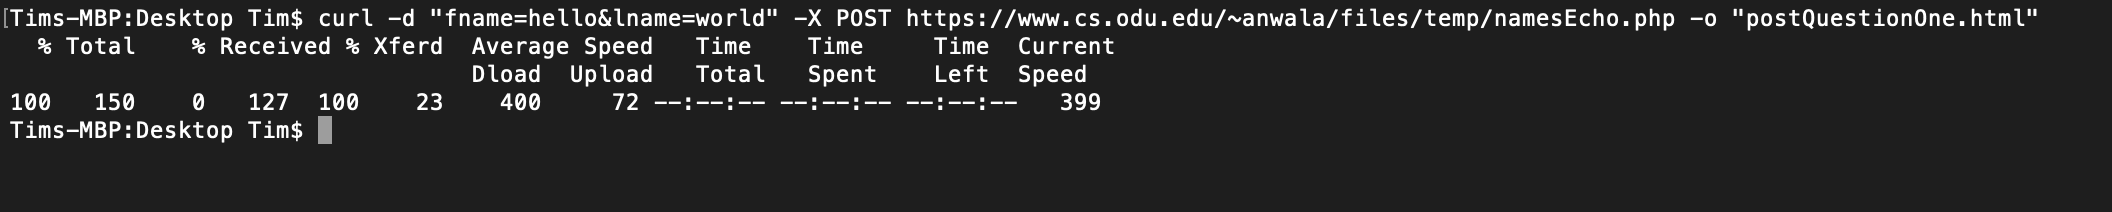
\includegraphics[width=\textwidth]{img1.png}

This produced the following output when the file "postQuestionOne.html" was opened.
\begin{center}
    Image 2: The HTML that was returned.
\end{center}
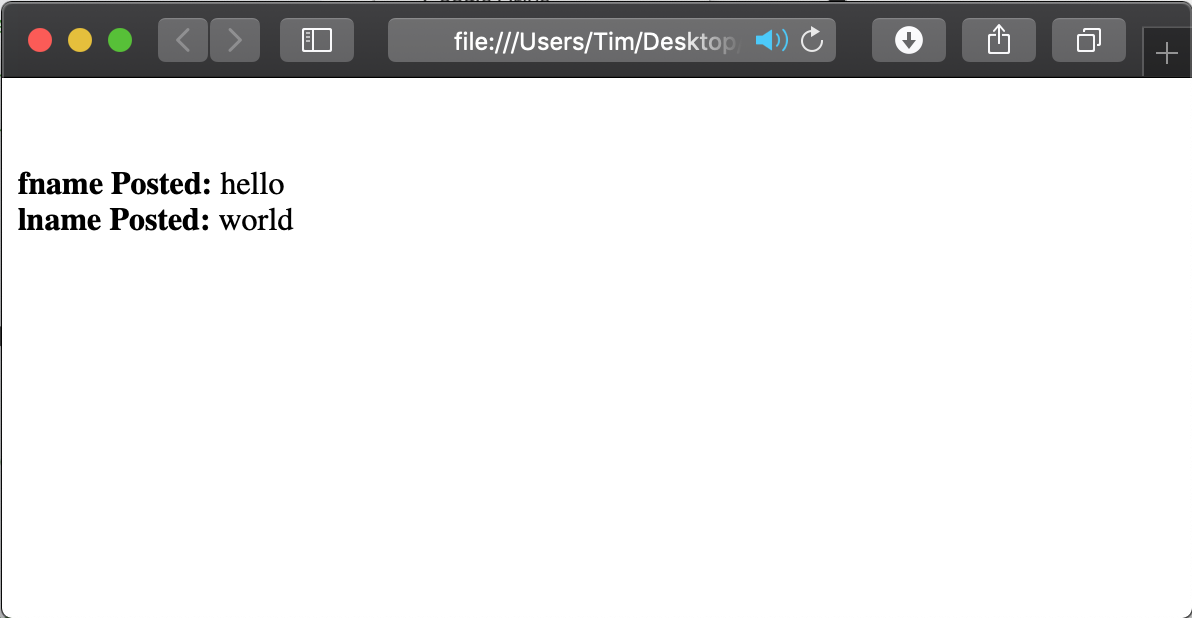
\includegraphics[width=\textwidth]{img2.png}

\end{homeworkProblem}
\begin{homeworkProblem}
Write a Python program that:
\begin{enumerate}
    \item takes as a command line argument a web page
    \item extracts all the links from the page
    \item lists all the links that result in PDF files, and prints out
     the bytes for each of the links.  (note: be sure to follow
     all the redirects until the link terminates with a "200 OK".)
    \item show that the program works on 3 different URIs, one of which
     needs to be: \newline http://www.cs.odu.edu/~mln/teaching/cs532-s17/test/pdfs.html
\end{enumerate}

\textbf{Solution} \newline
\part
TTake a web page as a command line argument. \newline
This is simple to do with the sys package in Python. However, I wanted to allow for some bad inputs in order to make this function reusable on future assignments. So I implemented the following program.

\begin{center}
    Listing 4: URL User Error Correction
\begin{mdframed}
\begin{lstlisting}[language=Python]
#Makes sure the address has an http or https
def ParseAddress(address, initialAddress = ""):
    if (address[0:8] != "https://" and address[0:7] != "http://"):
        if initialAddress != "":
            address = initialAddress + address
        else:
            address = "https://" + address
    return address
\end{lstlisting}
\end{mdframed}
\end{center}

This function checks if there is an http or https tag at the front of an inputted URL. If there is not such a tag, it will add one, either by just adding one and trying, or by using an optional parameter which would give an already known link to put onto the front.
\newline \newline 
\part
EExtract all of the links from the web page at the previous part's URL.\newline
This part actually has two sub-parts. 1. Open the web page, and 2. Extract all of the links. For the first part, urllib was used in a function called GetHTML with a parameter of the URL. This function simply returns the HTML code, and was written by using the URLLIB user documentation \cite{urllib-documentation}.\newline
Next, the BeautifulSoup library for Python was used to extract all of the "\textless a\textgreater" blocks. Once again, this is basic functionality and was done using the BeautifulSoup documentation \cite{beautiful-soup}. This left the program with the "\textless a\textgreater" blocks, but in order to check the links, there needs to be just the URL. This was done with some string manipulation using the standards for links in web pages.

\begin{center}
    Listing 5: URL Extraction From HTML.
\begin{mdframed}
\begin{lstlisting}[language=Python]
links = []
    for i in range(len(a_components)):
        start_bound = str(a_components[i]).find('href=\"')+6
        end_bound = str(a_components[i])[start_bound:].find('\"') + start_bound
        links.append(str(a_components[i])[start_bound : end_bound])
    return links
\end{lstlisting}
\end{mdframed}
\end{center}

In listing 5, a\_components is a list of every \textless a\textgreater block as a string. This snippet looks for the href tag in the \textless a\textgreater block and determines where the URL is in the string from there.
\newline \newline
\part
lList all the links that result in PDF files, and print out the bytes for each of the links.  (note: be sure to follow all the redirects until the link terminates with a "200 OK".)\newline
In the Slack for this class, Joshua Gahan confirmed that urllib already follows redirects. How to determine if a link actually led to a PDF had me stumped for a while, until I discovered a question by user gkennos on stack overflow about this very question. The answer is that in the header of a web page there is a "content-type" tag. So I wrote a function very similar to the GetHTML function described earlier called GetURLHeader, which returns the header as a Python dictionary, once again using the urllib library.\newline \newline
\part
aAfter all that, the program simply lists all of the links that it found! There is some additional code to show the status of checking the links because it takes a few seconds. The link status indicator does not show in the final output. Here is the output from three inputted URIs.

\begin{center}
    Image 3: Python output for given web page.
\end{center}
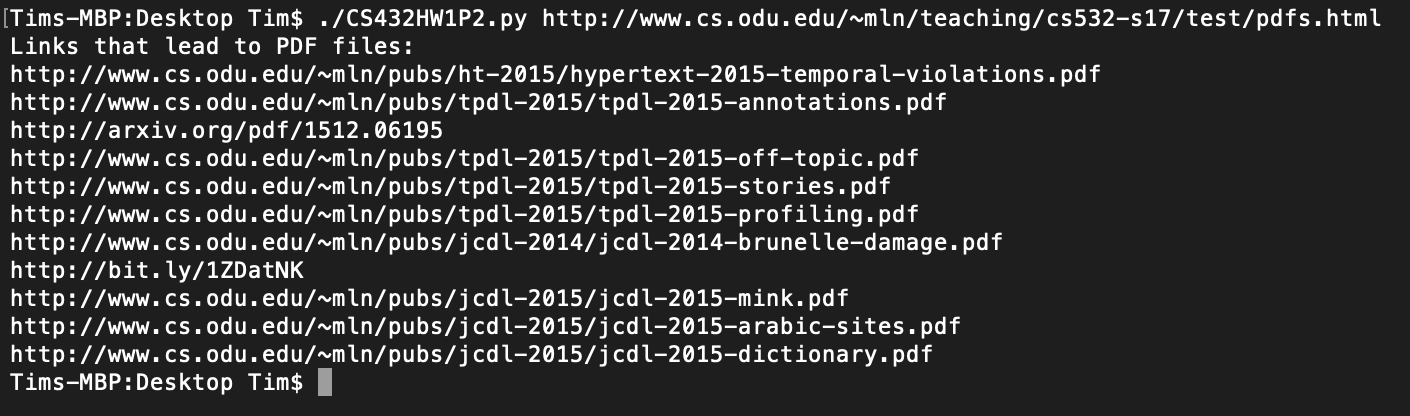
\includegraphics[width=\textwidth]{img3.png}
\begin{center}
    Image 4: Python output for a web page from a class I took a year ago.
\end{center}
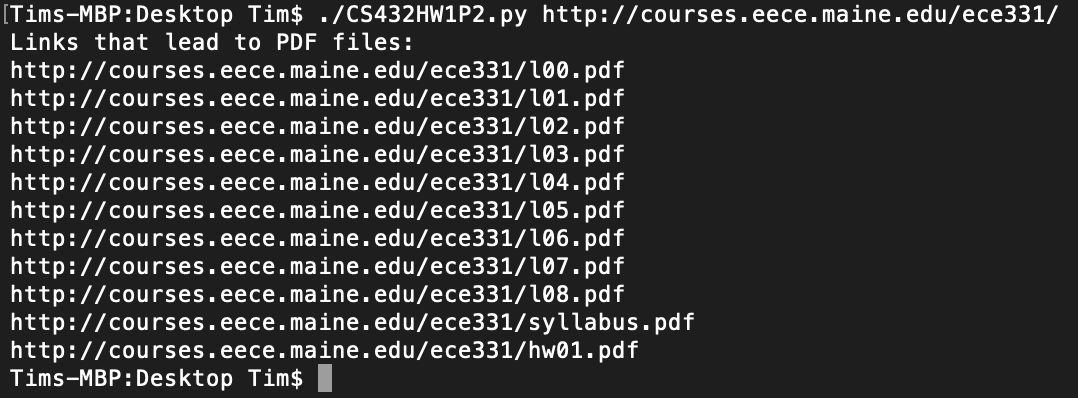
\includegraphics[width=\textwidth]{img4.png}
\begin{center}
    Image 5: Python output for the Wikipedia page on the PDF format.
\end{center}
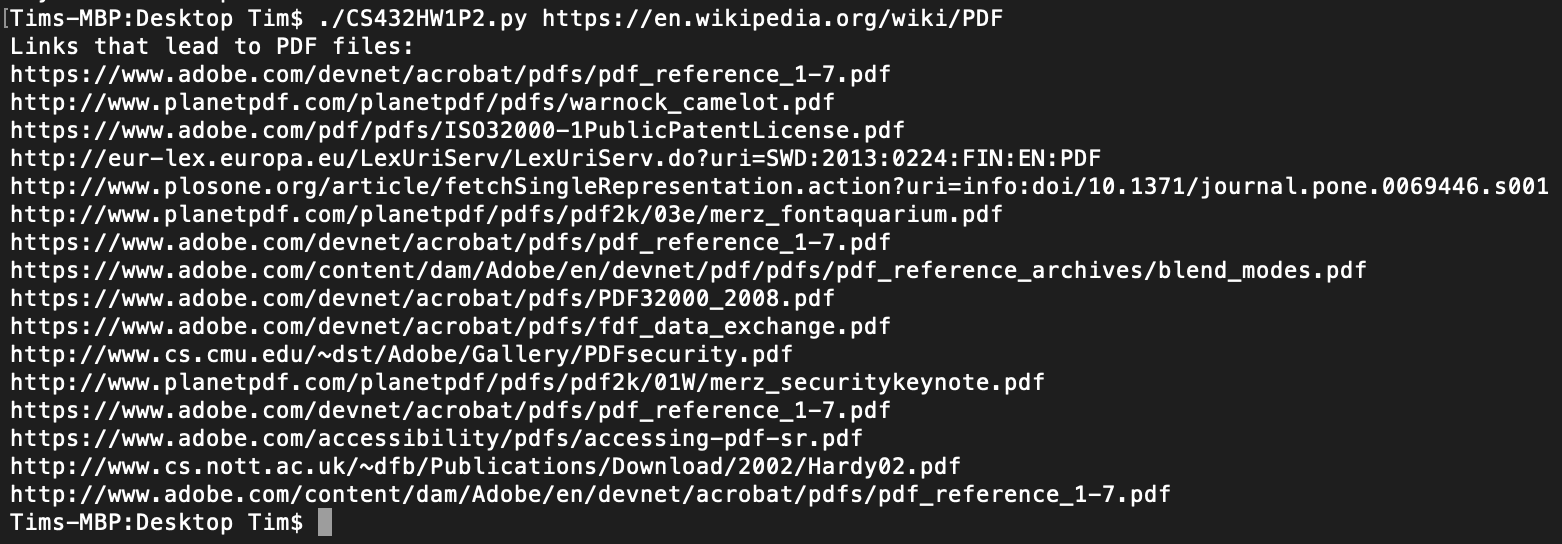
\includegraphics[width=\textwidth]{img5.png}

\end{homeworkProblem}
\begin{homeworkProblem}
Consider the "bow-tie" graph in the Broder et al. paper:
    
    http://snap.stanford.edu/class/cs224w-readings/broder00bowtie.pdf

    Many have found this link useful: 
    https://www.harding.edu/fmccown/classes/archive/comp475-s13/web-structure-homework.pdf
    Now consider the following graph:\newline
    A --\textgreater B \newline
    B --\textgreater C\newline
    C --\textgreater D\newline
    C --\textgreater A\newline
    C --\textgreater G\newline
    E --\textgreater F\newline
    G --\textgreater C\newline
    G --\textgreater H\newline
    I --\textgreater H\newline
    I --\textgreater K\newline
    L --\textgreater D\newline
    M --\textgreater A\newline
    M --\textgreater N\newline
    N --\textgreater D\newline
    O --\textgreater A\newline
    P --\textgreater G \newline
    
    For the above graph, give the values for:

    IN,
    SCC, 
    OUT, 
    Tendrils, 
    Tubes, and
    Disconnected
\newline \newline
\textbf{Solution}\newline
To solve this puzzle I started by writing each letter in order twice, with all of the connections being drawn from left to right. Note that I assume that J exists despite lack of any information about its existence.

\begin{center}
    Image 6: Method used to organize the links.
\end{center}
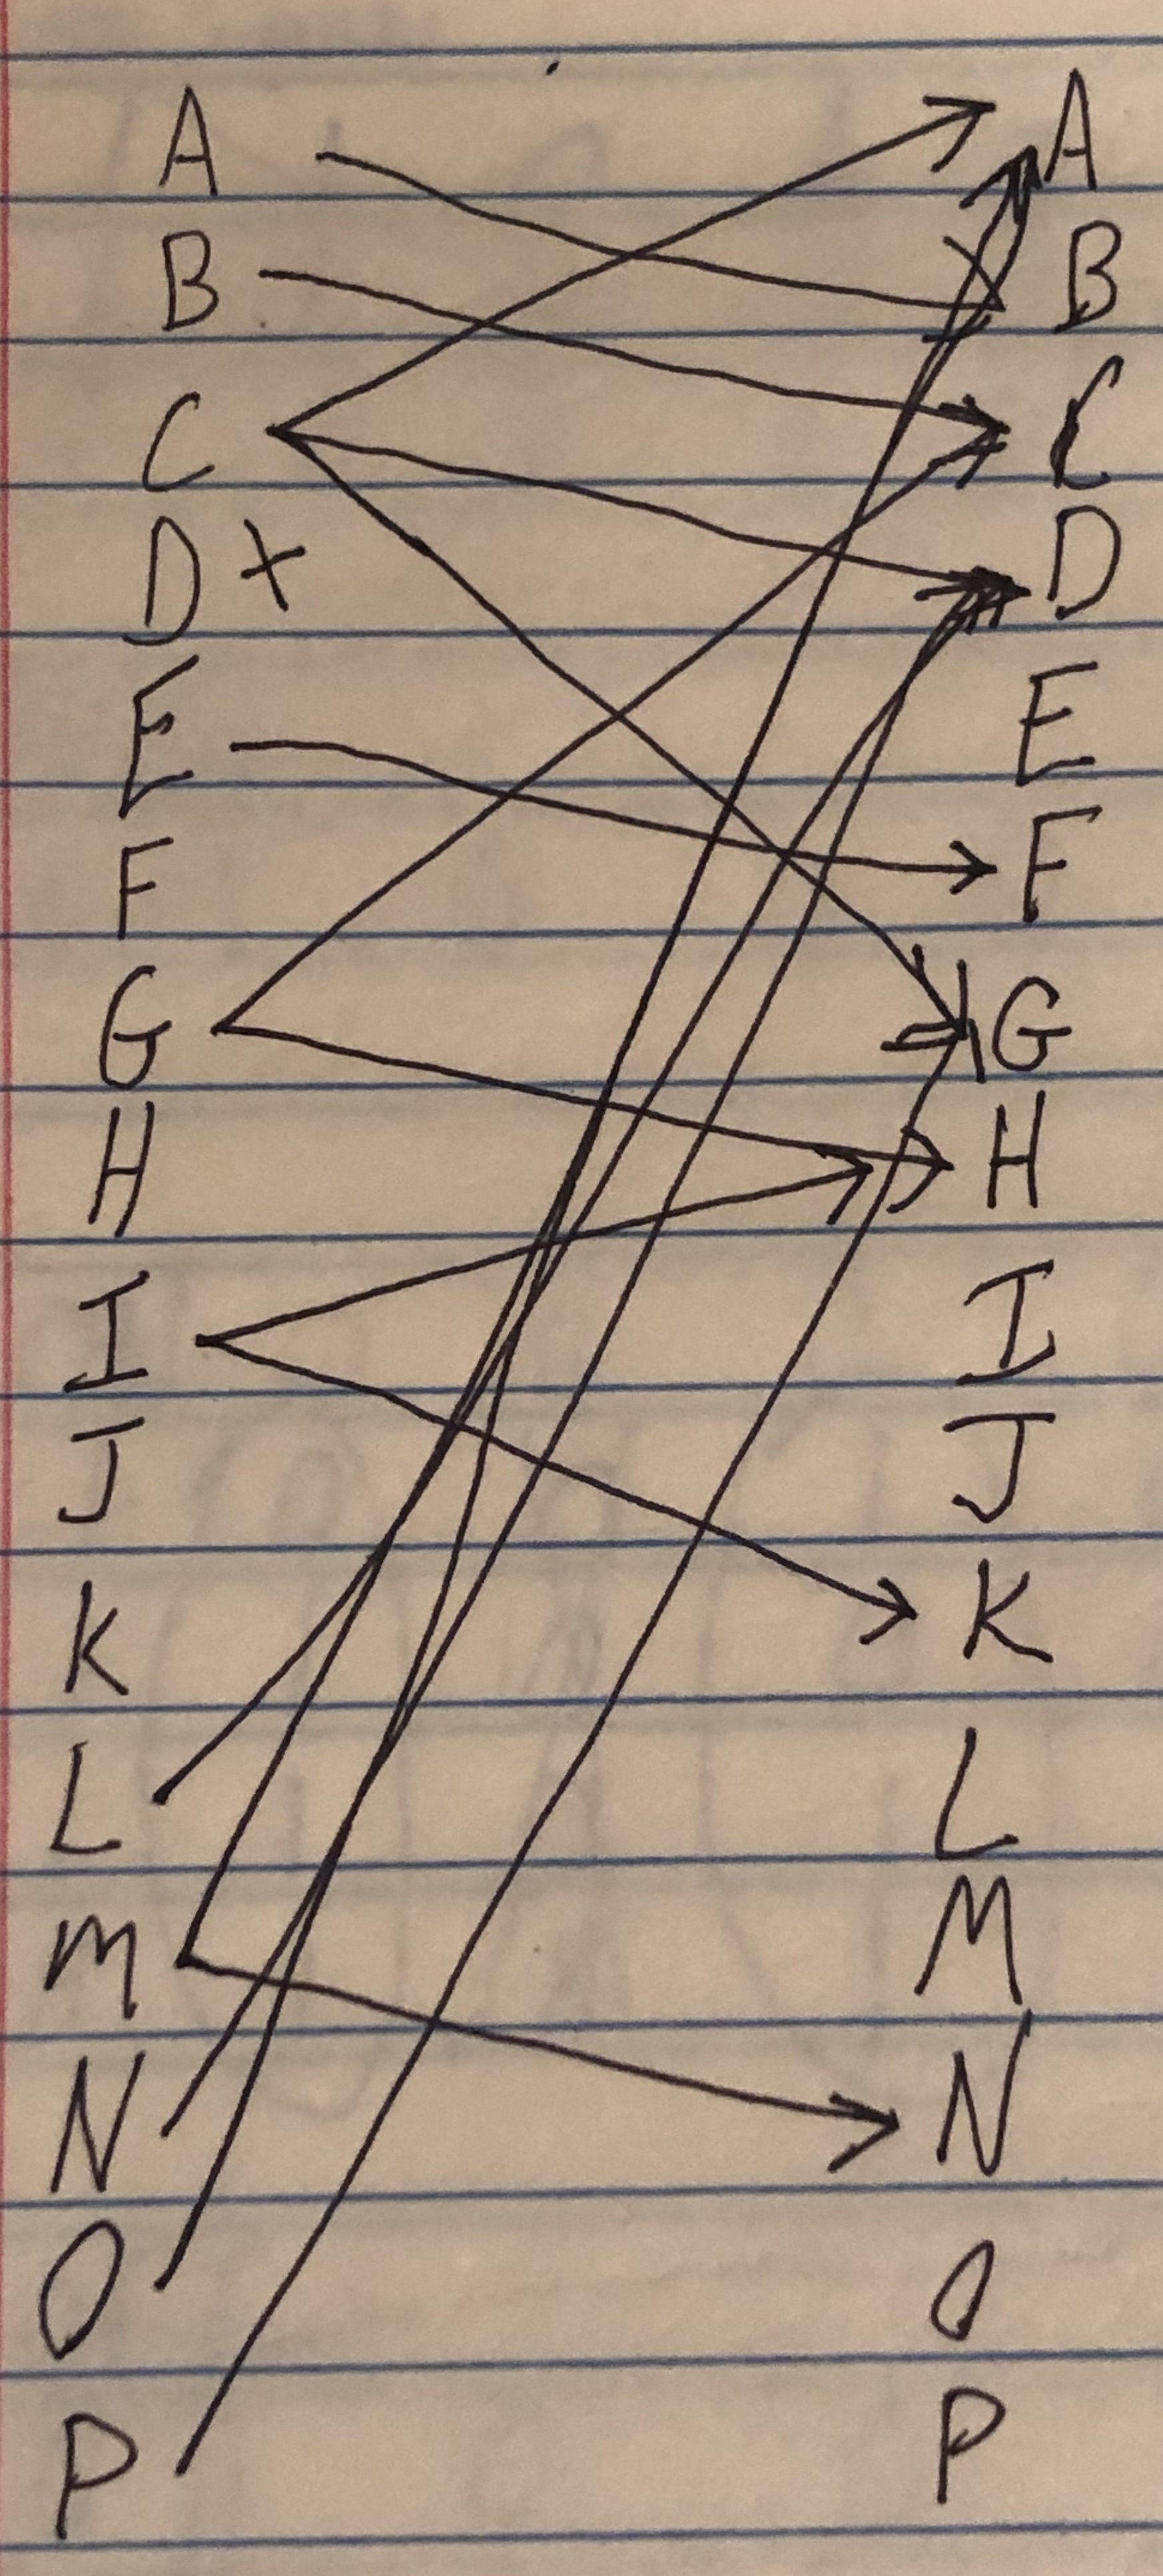
\includegraphics[width=250pt]{img6.jpg}

Using this I was able to get a good sense of what was what. After one test-draw, I was able to determine a good clean final version of the graph. The in nodes all lead into the SCC. SCC all lead to each other. End are all links out of 
\begin{center}
    Image 7: The final graph.
\end{center}
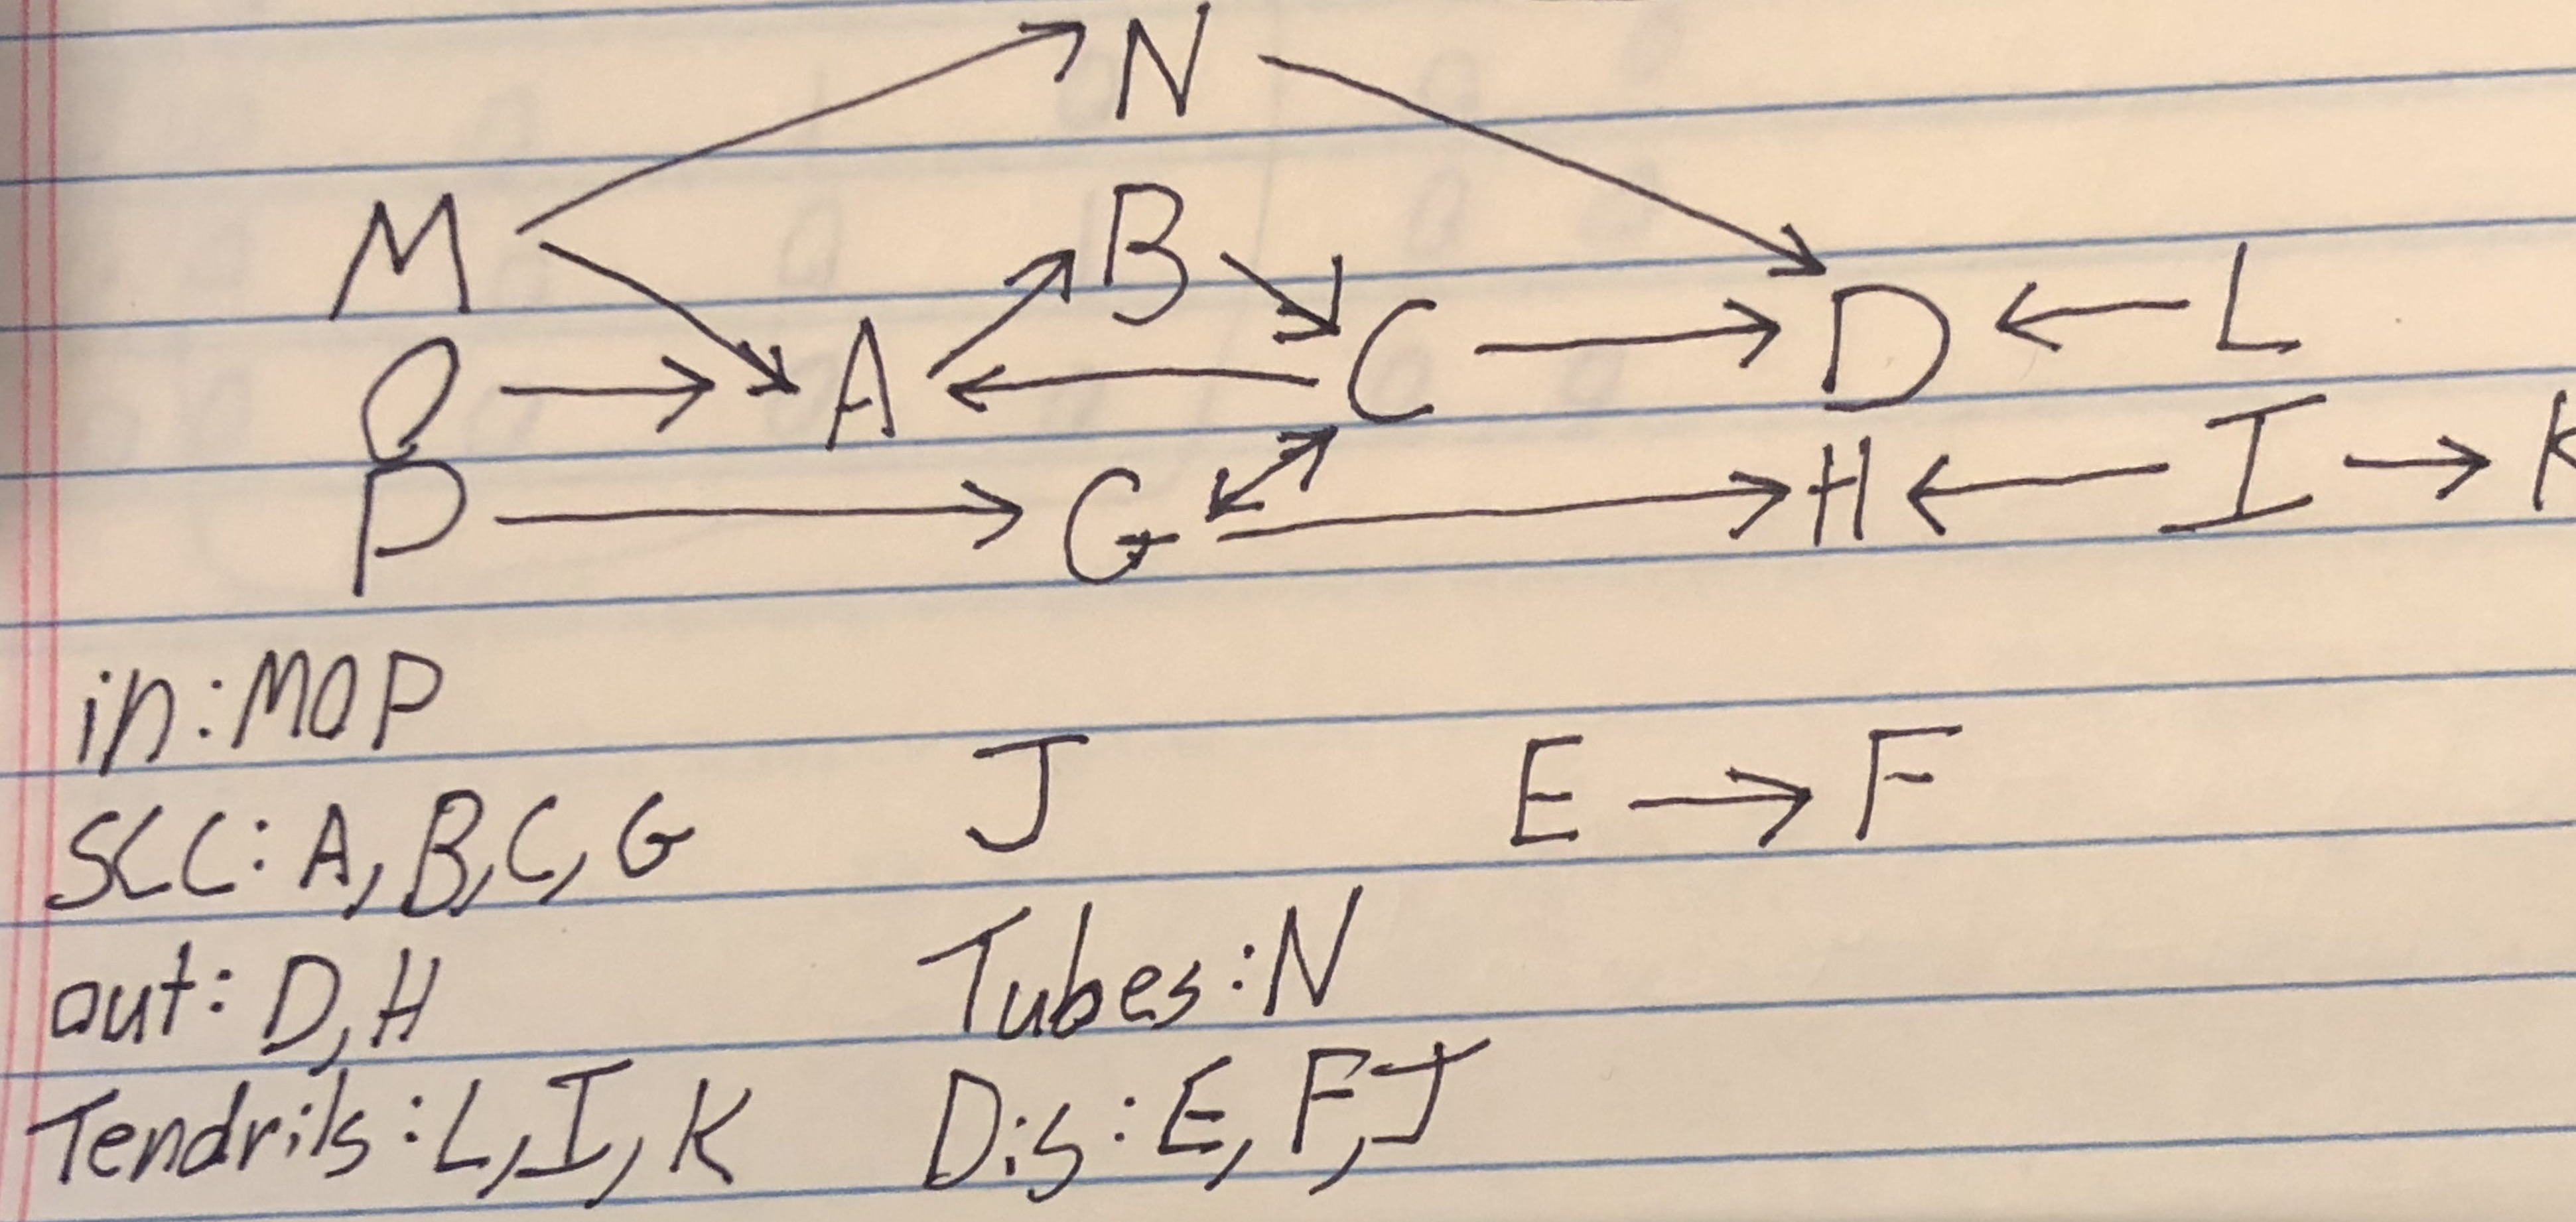
\includegraphics[width=\textwidth]{img7.jpg}

The nodes are organized as follows:\newline
IN: M, O, P\newline
SCC: A, B, C, G\newline
OUT: D, H\newline
TENDRILS: L, I, K\newline
TUBES: N\newline
DISCONNECTED: E, F, J\newline

\end{homeworkProblem}

\bibliographystyle{IEEEtran}
\bibliography{bibliography.bib}
\end{document}
